\clearpage
\section{Reinforcement Learning for Sequential Decision-Making}
\label{sec:reinforcement_learning}

\subsection*{Introduction}
Reinforcement Learning (\textbf{RL}) is a way for an agent to learn by trying actions and getting feedback. If the action helps, the agent gets a better reward. If not, it learns and tries again. That simple loop makes RL a good fit for tasks that happen step by step, like moving an endoscope, keeping the view stable, or controlling a snare \cite{sutton2018reinforcement}.

In this work, RL is not just theory in a textbook. It is the idea behind an agent that must act in a messy, changing scene and still stay safe. We use modern policy methods, especially \textbf{Proximal Policy Optimization (PPO)}, because they are stable and work well with neural networks \cite{schulman2017ppo}. Classic deep RL results such as \textbf{DQN} and \textbf{AlphaGo} show how far the field has come \cite{mnih2015dqn,silver2016alphago}.

\begin{figure}[h]
\centering
\fbox{\parbox[b][3.8cm][c]{0.9\linewidth}{\centering Placeholder: RL overview showing agent, environment, state, action, and reward}}
\caption{Main RL components and feedback loop (placeholder).}
\label{fig:rl_components}
\end{figure}

\subsection{The RL Loop}
The RL loop is easy to remember: the agent sees a \textbf{state}, chooses an \textbf{action}, and gets a \textbf{reward}. Then the environment changes, and the next state appears. This repeats many times. The goal is not to win one step, but to collect the best total reward over time.

For our project, this loop matters because the best action now may depend on what happened a few frames ago. A small move can make the next image clearer, or a wrong move can hide the lesion. RL helps the agent learn that timing matters.

\begin{figure}[h]
\centering
\fbox{\parbox[b][3.5cm][c]{0.9\linewidth}{\centering Placeholder: agent--environment loop / MDP diagram}}
\caption{Agent--environment interaction as an MDP (placeholder).}
\label{fig:mdp_loop}
\end{figure}

\subsection{Key Concepts}
\begin{itemize}
	\item \textbf{State:} what the agent knows right now, such as images, scope position, or tool state.
	\item \textbf{Action:} what the agent can do, such as move, stop, open the snare, or apply energy.
	\item \textbf{Reward:} a number that says how good the last action was.
	\item \textbf{Policy:} the agent's behaviour rule, usually written as \(\pi\).
	\item \textbf{Return:} the total future reward, for example $G_t = r_t + \gamma r_{t+1} + \dots$.
	\item \textbf{Value:} a guess of how good a state or action may be in the future.
\end{itemize}

These words are small, but they carry the whole chapter. If the state is poor, the action may be poor too. If the reward is wrong, the agent may learn the wrong lesson. So the definitions are not just formalities; they shape the whole system.

\subsection{Markov Decision Process}
We model the problem as a \textbf{Markov Decision Process} (MDP). An MDP has five parts: states, actions, transitions, rewards, and a discount factor. The Markov idea says that the next step depends mostly on the current state and current action, not on the full history.

This is not a perfect description of the real world, but it is a useful one. It keeps the problem clean enough to train an agent, while still matching how procedural tasks work in practice \cite{sutton2018reinforcement}.

\begin{figure}[H]
\centering
\setlength{\fboxsep}{4pt}% padding between image and frame
	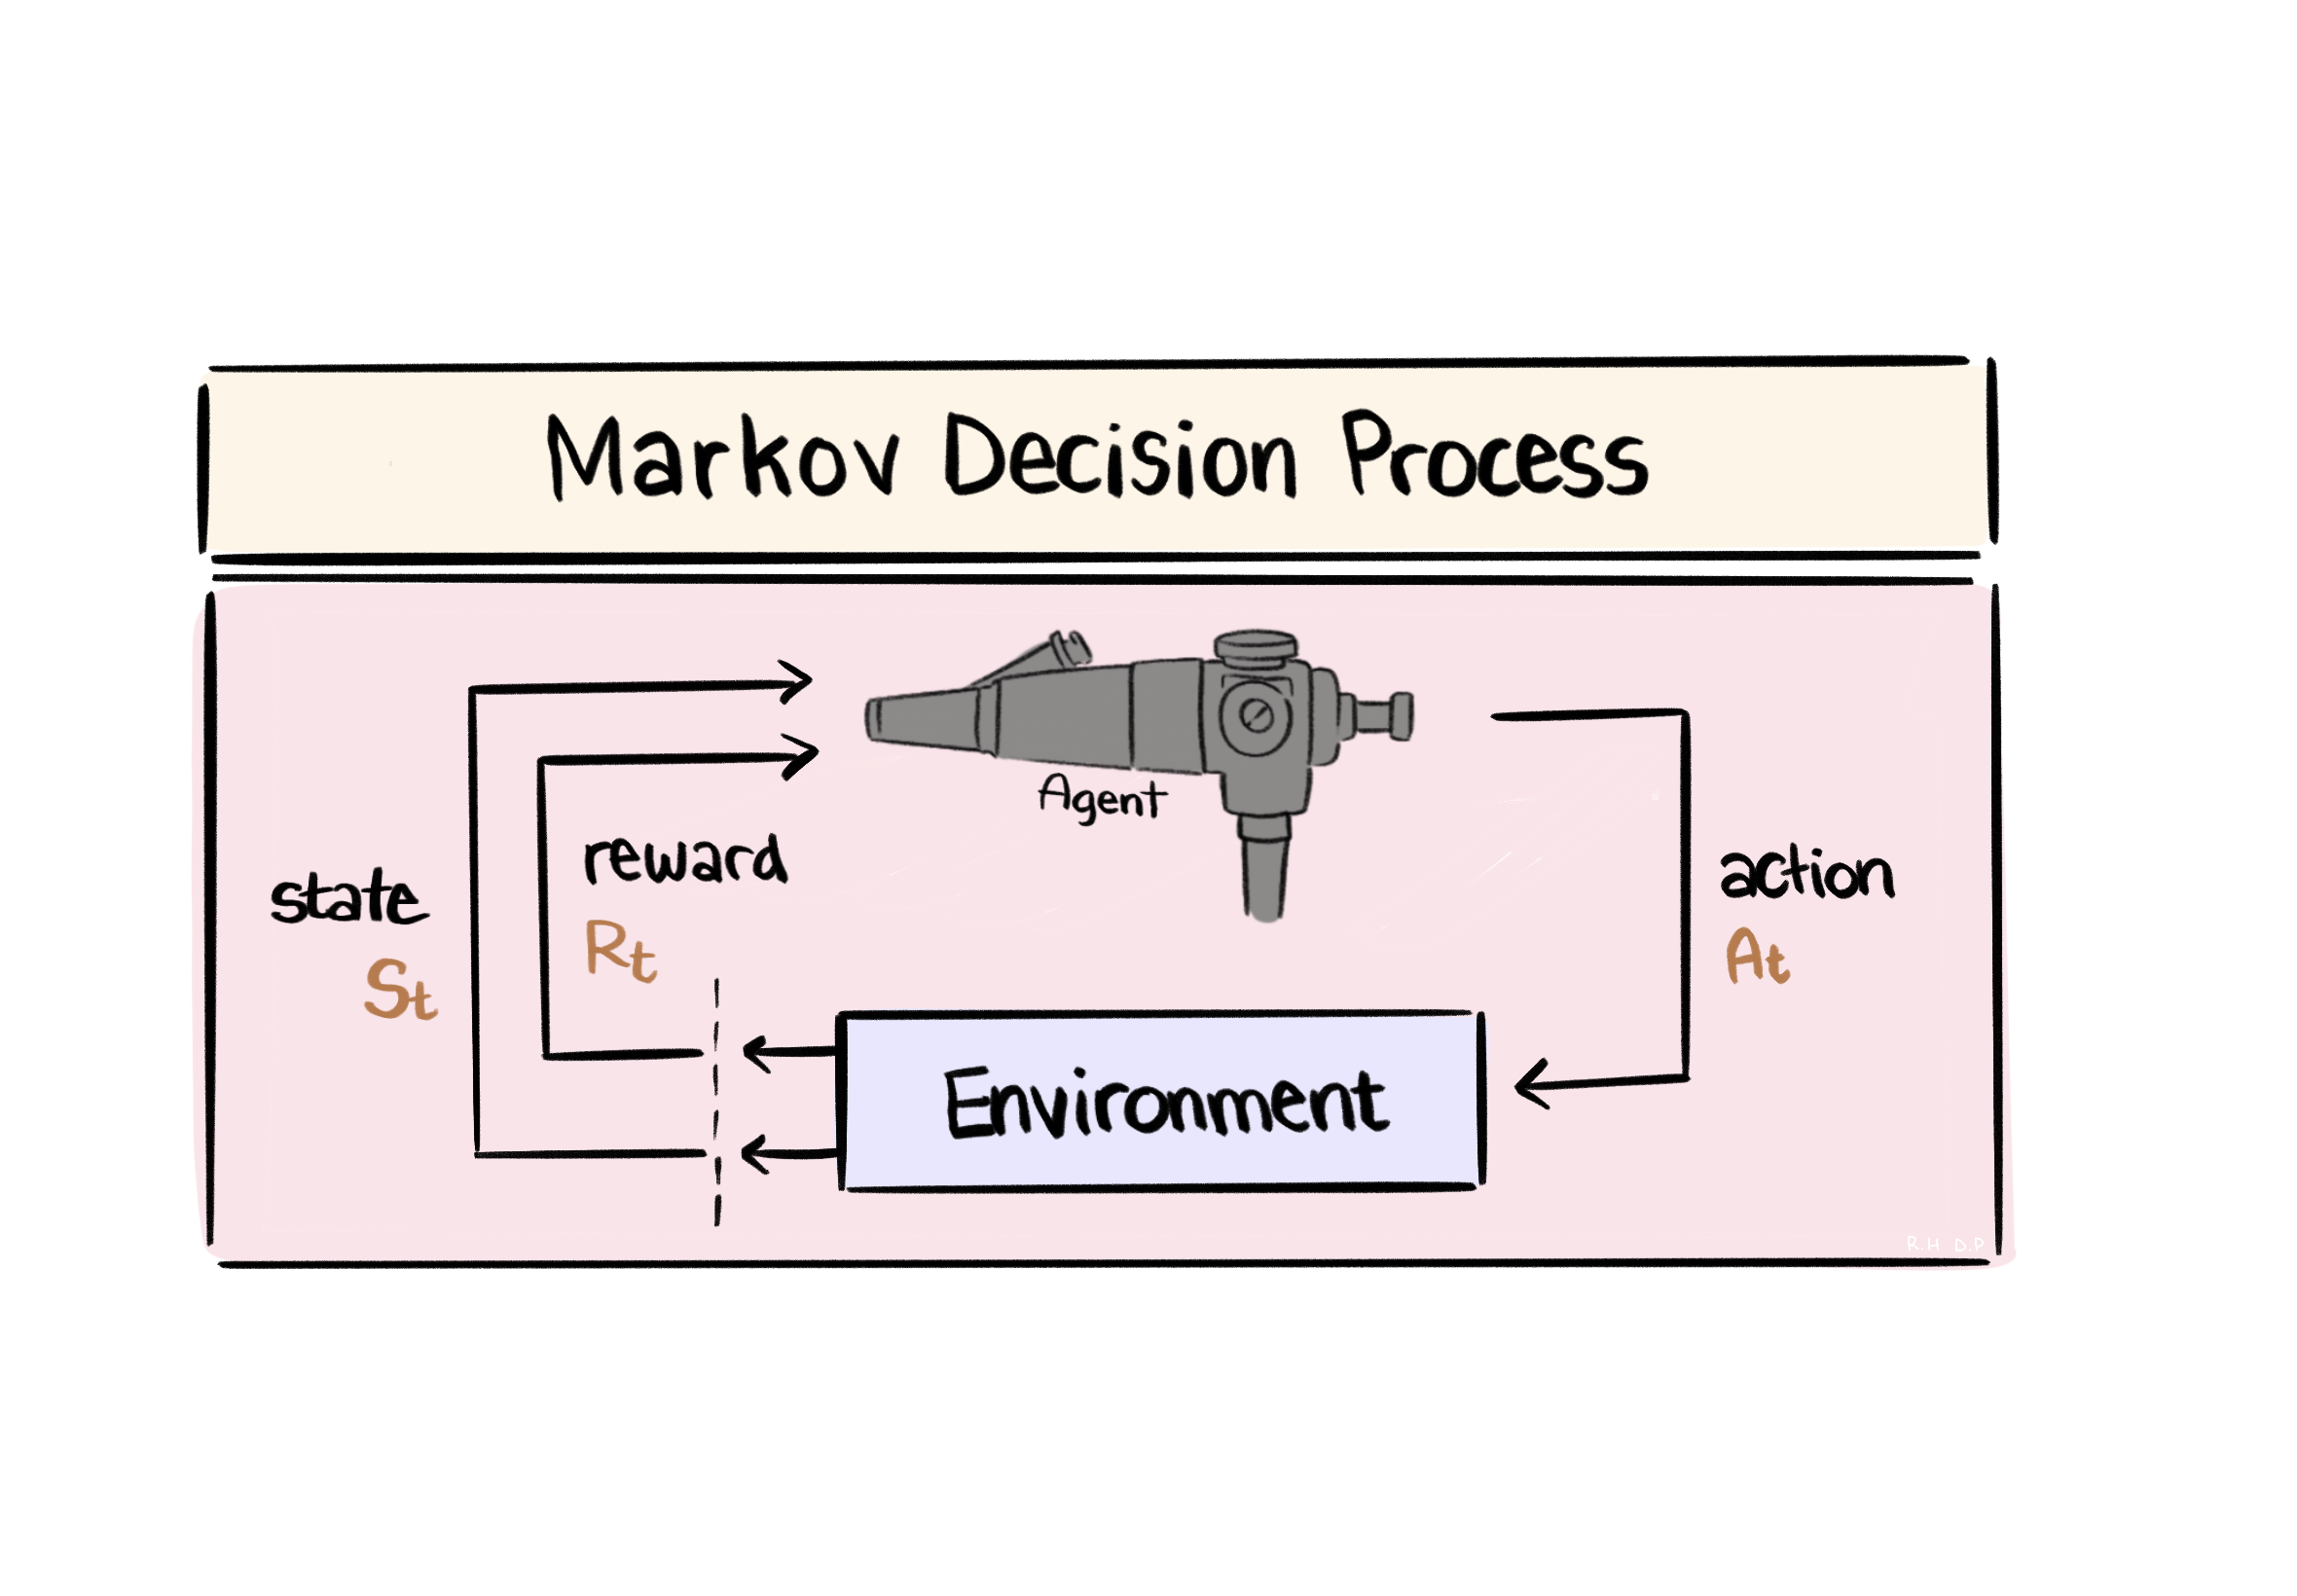
\includegraphics[width=0.8\linewidth,trim=0 6cm 0 6cm,clip]{assets/diagram-MDP.png}%
\caption{State transition and reward flow in an MDP.}
\label{fig:mdp_state_transition}
\end{figure}

\subsection{Value and Policy Methods}
There are two main ways to solve an RL problem. The first is \textbf{value-based learning}. Here the agent learns how good each action is. The second is \textbf{policy-based learning}. Here the agent learns the action rule directly.

Value methods such as Q-learning are simple and useful, especially when the action space is small. Policy methods are often better for continuous control, where the agent needs to steer smoothly instead of choosing from a short list of actions. That is why this work focuses on policy methods and actor-critic ideas, especially PPO \cite{schulman2017ppo}.

\begin{figure}[h]
\centering
\fbox{\parbox[b][3.4cm][c]{0.9\linewidth}{\centering Placeholder: value-based vs policy-based RL comparison}} 
\caption{Two main RL families: value-based and policy-based (placeholder).}
\label{fig:rl_taxonomy}
\end{figure}

\subsection{Why PPO Fits This Work}
PPO is popular because it keeps training stable. It updates the policy in small steps instead of making one big jump. That is helpful when the agent works in a noisy visual setting, where a big update could make the behaviour worse very quickly.

In simple terms, PPO tries to improve the agent without letting it become too adventurous at once. That is a good match for endoscopy, where we want progress, but not chaos. The policy should learn smooth and reliable behaviour, not dramatic surprises.

\begin{figure}[h]
\centering
\fbox{\parbox[b][3.6cm][c]{0.9\linewidth}{\centering Placeholder: PPO training loop with policy, critic, and clipped update}}
\caption{PPO training loop and clipped policy update (placeholder).}
\label{fig:ppo_loop}
\end{figure}

\subsection{Reward Design and Safety}
In a medical setting, reward design is a big deal. A bad reward can lead to odd behaviour. The agent may chase the score instead of the real goal. So rewards should be simple, clear, and tied to safe actions.

Useful ideas include:
\begin{itemize}
	\item \textbf{Reward shaping:} give small feedback during the task, not only at the end.
	\item \textbf{Penalties:} reduce reward for unsafe moves or bad tool contact.
	\item \textbf{Human review:} let clinicians check whether the behaviour looks sensible.
	\item \textbf{Simulation first:} train in a virtual setting before any real-world test.
\end{itemize}

\begin{figure}[h]
\centering
\fbox{\parbox[b][3.2cm][c]{0.9\linewidth}{\centering Placeholder: reward design diagram showing progress reward and safety penalties}}
\caption{Example reward design for safe RL (placeholder).}
\label{fig:reward_design}
\end{figure}

\subsection{Exploration}
RL also needs exploration. The agent must try new things to improve, but it should not take wild risks all the time. A small amount of exploration is good; too much is noisy; too little makes learning slow.

In practice, we often use controlled exploration such as action noise or epsilon-style randomness. In safety-critical tasks, simulation is the place to explore more freely, because the agent can fail there without harming a patient.

\subsection{RL in Endoscopy}
RL is useful in endoscopy because the task is sequential and visual. The agent may need to move the scope, keep the target in view, and decide when to act. This is not a single-frame problem. It is more like a short story: one move changes the next scene, and the next scene changes the next decision.

Recent work in surgical and medical robotics shows the same pattern: learning in simulation, safety constraints, and sim-to-real transfer are the big challenges \cite{qian2023arxiv,pore2022iros,corsi2023arxiv,ou2023lra,surrol2021arxiv}.

\begin{table}[h]
\centering
\caption{Simple view of RL methods used in this chapter}
\begin{tabular}{|l|l|l|}
\hline
\textbf{Method} & \textbf{Main idea} & \textbf{Why it helps} \\ \hline
Q-learning & Learn action values & Simple for discrete actions \\ \hline
Actor-critic & Policy + critic & More stable learning \\ \hline
PPO & Safe policy updates & Good for continuous control \\ \hline
\end{tabular}
\label{tab:rl_methods_short}
\end{table}

\subsection{Summary}
RL gives us a clean way to teach an agent step by step. In this project, the agent must learn safe and useful actions for navigation and extraction, so we focus on policy-based methods, especially PPO. The next chapter explains PPO in more detail.

